\documentclass{standalone}
\usepackage{tikz}
\usepackage{ctex,siunitx,ninecolors}
\setCJKmainfont{Noto Serif CJK SC}
\usepackage{tkz-euclide}
\usepackage{amsmath}
\usepackage{wasysym}
\usetikzlibrary{patterns, calc}
\usetikzlibrary {decorations.pathmorphing, decorations.pathreplacing, decorations.shapes,}
\begin{document}
\small
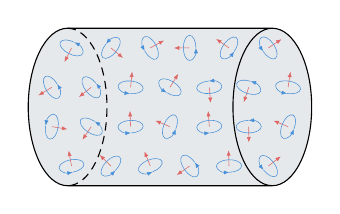
\begin{tikzpicture}[>=latex,scale=1]
  \draw[fill=cyan!10!gray!20,draw](1.3,1)--(-1.3,1)arc(90:270:0.5 and 1.0)--(1.3,-1)(1.3,0)ellipse(0.5 and 1.0);
  \draw[densely dashed] (-1.3,1)arc(90:-90:0.5 and 1.0);
  \foreach \x in {-1.25,-0.75,-0.25,0.25,0.75,1.25}
  {
    \foreach \y in {-0.75,0.75}
    {
      \begin{scope}[xshift=\x cm,yshift=\y cm,rotate=360*rnd]
      \draw[very thin,arrows={-Latex[scale=0.5]},red6](0,0)--++(0.2,0);
      \draw[very thin,azure6,,arrows={-Latex[scale=0.5]}](-0.08,0)arc(-180:180:0.08 and 0.16);
      \end{scope}
    }
  }
  \foreach \x in {-1.5,-1.0,-0.5,0,0.5,1.0,1.5}
  {
    \foreach \y in {-0.25,0.25}
    {
      \begin{scope}[xshift=\x cm,yshift=\y cm,rotate=360*rnd]
      \draw[very thin,arrows={-Latex[scale=0.5]},red6](0,0)--++(0.2,0);
      \draw[very thin,azure6,,arrows={-Latex[scale=0.5]}](-0.08,0)arc(-180:180:0.08 and 0.16);
      \end{scope}
    }
  }

\end{tikzpicture}
\end{document}